\section{29 Aug 23 - Notes: Simple Harmonic
Oscillator}\label{aug-23---notes-simple-harmonic-oscillator}

\subsection{A Linear Restoring Force}\label{a-linear-restoring-force}

The SHO model, as we will see, is the root of many more sophisticated
models in physics -- across many subdisciplines. There's a reason for
this. The SHO is a simple model that captures the essence of many
physical systems. It is a mathematical model for a ``linear restoring
force''. Such a force gives rise to local stability, that is, a tendency
for the system to return to a stable equilibrium position. The richness
of this statement is not entirely clear, but we will see that it is a
very powerful idea, that is related to to energy minimization, and the
idea of a potential energy function.

A linear restoring force is simply one in which the size of the force is
in direct proportion to some displacement and is directed opposite to
the displacement. For example, a coiled spring exerts (rooughly) a
linear restoring force. If you pull on a spring, the spring exerts a
force on your hand that is proportional to the distance you pull the
spring. It is directed opposite to the direction you pull.

In 1D, we can write this as:

\[F_{\rm spring} = -kx\]

where \(k\) is the spring constant. The negative sign indicates that the
force is directed opposite to the displacement, and \(x\) is the
displacement from the equilibrium position. As we are going to consider
more general motion, we can abstract this concept of a linear restoring
force to three dimensions, and write:

\[\vec{F}_{\rm spring} = -k \Delta \vec{x}\]

where \(\Delta \vec{x}\) is the displacement vector from the equilibrium
position.

\subsection{The SHO mathematical
model}\label{the-sho-mathematical-model}

We have seen that the canonical one-dimensional harmonic oscillator is
described with the following \textbf{2nd order linear} differential
equation:

\[m\ddot{s} = -k{s}\]

where \(s\) represents the distance from the oscillator's equilibrium
position. It's important to note that this model for a linear restoring
force gives rise to at \textbf{second order} differential equation. As
you will see, there would be no ability for cycles or recurrent behavior
without two dimensions (the two dimensions here are the position, \(s\),
and velocity of the oscillator, \(\dot{s}\)). It is also important that
the differential equation is \textbf{linear}.

\subsubsection{Linearity of differential
equations}\label{linearity-of-differential-equations}

This is something that is easy to confuse because we use the term
\textbf{linear} in different ways at different times. In many cases this
prompts us to think of a line, so that we might think the only linear
differential equations are ones where the variable of interest (in this
case the position of the oscillator) appears only \emph{linearly} in the
equation.

So you might think that Nth order differential equations of the form:

\[\dfrac{d^n x}{dt^n} = c\;x\]

are the only ones that are linear. \emph{Note for the harmonic
oscillator \(n=2\); \(c<0\).}

\textbf{That is not the case and this is key.}

The linearity refers to the fact that we can write the differential
equation as a \textbf{linear combination of the derivatives}.

:::\{admonition\} Linear Differential Equations :class: note

So an \(N\)th linear differential equation (e.g., for position and time)
can have the general form:

\[\sum_{i=0}^N a_i(t)\dfrac{d^ix}{dt} = f(t)\]

where \(\dfrac{d^ix}{dt}\) is the \(i\)th derivative of \(x\) (e.g.,
\(i=0\), \(\dfrac{d^0x}{dt}=x\); \(i=1\),
\(\dfrac{d^1x}{dt}=\dfrac{dx}{dt}\)) The coefficients are allowed to
depend explicitly on time (i.e., \(a_i(t)\); you have probably seen
\emph{constant coefficients} in the past (where
\(\dfrac{da_i(t)}{dt}=0\), i.e., \(a_i(t) =\) constant). In addition, as
you can explore later, the system can be driven by a function that
depends only on time (e.g., some forcing function, \(f(t)\)). :::

\subsubsection{Why does linearity
matter?}\label{why-does-linearity-matter}

Because much of nature can be modeled with linear differential equations
(or approximately so) and linear differential equations have really nice
solution properties. *The solutions to linear differential equations are
\textbf{holonomic functions}. This is just a fancy word for functions
you know like polynomials, sine, cosine, exponentiale, and some special
functions (e.g., Airy, Bessel, hypergeometric). But these solutions are
really important because they are smooth as are their derivatives, so
they have really nice properties.

In many cases, we can lean on strong properties derived from linearity:

\begin{itemize}
\tightlist
\item
  \href{https://en.wikipedia.org/wiki/Cauchy\%E2\%80\%93Kowalevski_theorem}{Uniqueness}:
  If we find a solution to the differential equation and it satisfies
  the boundary/initial conditions, we are guaranteed that this is the
  only solution.
\item
  Linear combinations: The linear nature of the differential equation
  means linear combinations of general solutions are unchanged. We can
  build solutions from known general solutions.
\end{itemize}

```\{admonition\} The Cauchy-Kowaleski theorem :class: note This theorem
is typically called the Cauchy theorem (or the uniqueness theorem) for
\href{https://en.wikipedia.org/wiki/Augustin-Louis_Cauchy}{Augustin
Louis-Cachy}, a French mathematician who contributed much to the field
of complex analysis. However, Cauchy only proved this theorem in a
special case. A Russian Mathematician,
\href{https://en.wikipedia.org/wiki/Sofya_Kovalevskaya}{Sofya
Kovalevskaya}, who was the first woman to earn a PhD in Mathematics
(earned 1874, University of Göttingen), proved the theorem, in general,
in her dissertation.

\textbf{So, it is really the ``Kovalevskaya-Cauchy'' theorem.}

\begin{verbatim}

### General Solution to the SHO

We can start with the differential equation:

$$\ddot{x} = -\omega^2 x$$

where $x$ is the position relative to equilibrium and $\omega^2 = k/m$. We know this is a linear, second-order ODE, so we expect the solutions to be [holonomic functions](https://en.wikipedia.org/wiki/Holonomic_function) - that is, many of the functions we have seen before. Moreover, we need something that when we take two derivatives, we get the same functions back.

*This is a key to suggest $\sin$ and $\cos$ as our proposed linear combination.*

Now, we have to decide how to do that. Because **ANY** linear combination is a good starting guess, but not all of them a reasonable guesses. How do we decide? 

```{admonition} Discussion Question
:class: tip


Below are several choices of potential general solution guesses, called "ansatz" in many books and classes. 

Which of them will work for us? How do you know? Demonstrate that one solution you chose works.

$$x(t) = A\cos(\omega t)$$
$$x(t) = B\sin(\omega t)$$
$$x(t) = A\cos(\omega t)+B\sin(\omega t)$$
$$x(t) = B\sin(\omega t+ \phi_B)$$
$$x(t) = \sum_i^N A_i\cos(\omega_i t) + B_i\sin(\omega_i t)$$

**What other general solution forms will work?** 
\end{verbatim}

```\{dropdown\} Hint Can you think of other functions that when you take
two derivatives, you get the same function back with a sign change?

What if the function were complex (recall: \(i^2 = -1\))?

\begin{verbatim}

### Particular Solutions

Let's pick two general solutions. Notice that both have two unknown constants. We can use the initial conditions to determine the values of these constants, and thus our particular solutions. 

$$x(t) = A\cos(\omega t) + B\sin(\omega t)$$

$$x(t) = C\sin(\omega t + \phi_C)$$

To determine a particular solution is to solve for the **trajectory** of the system given a set of initial conditions. You can think about a falling object, but any physical system that is evolving in time will have a trajectory in the general sense of various changing observable quantities. We will revisit this idea later once we make the connection to [Dynamical Systems](https://en.wikipedia.org/wiki/Dynamical_system).

#### Find a particular solution

For an SHO ($\omega=\omega_0 = 1$) that is pulled to a point $x_0$ and let go at $t=0$, let's find the particular solutions using both general forms (they will give us this). 

$$x_1(t) = x_0\cos(\omega_0 t)$$
$$x_2(t) = x_0\sin(\omega_0 t + \pi/2)$$
$$x_2(t) = -x_0\sin(\omega_0 t + 3\pi/2)$$


```python
import numpy as np
import matplotlib.pyplot as plt

#################################
# Adjust code to fit your needs #
#################################

t = np.arange(0,10,0.1)
x0 = 1
omega0 = 1

x1 = x0*np.cos(omega0*t)
x2a = x0*np.sin(omega0*t + np.pi/2) + 1 # to make it offset
x2b = -x0*np.sin(omega0*t + 3*np.pi/2) - 1 # to make it offset

plt.plot(t,x1)
plt.plot(t,x2a)
plt.plot(t,x2b)
\end{verbatim}

\begin{verbatim}
[<matplotlib.lines.Line2D at 0x11518d510>]
\end{verbatim}

\begin{figure}
\centering
\pandocbounded{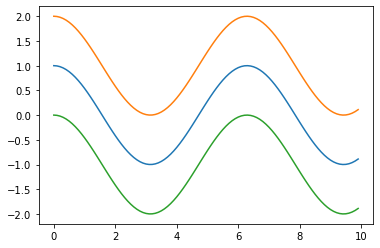
\includegraphics[keepaspectratio,alt={png}]{../images/notes-SHO_notes-SHO_tmp_7_1.png}}
\caption{png}
\end{figure}

\subsection{Resources}\label{resources}

Here are scans of four sections of four books (that you can look over at
my office, or find elsewhere) that are useful for our study of the SHO
and will help you with your project ideas and plans.

\emph{Sorry for the potato quality, and apparently the orientations,
which I corrected but github refuses to keep the same orientation. I
will do better next class and try to fix these later.}

\begin{itemize}
\tightlist
\item
  \href{https://github.com/dannycab/phy415msu/blob/main/MMIPbook/assets/pdfs/scans/Boas_ODEs_8.5.pdf}{Boas,
  Mathematical Methods, Sec 8.5}

  \begin{itemize}
  \tightlist
  \item
    This section goes into all the math (in general) for ODEs like the
    SHO, which are second order (\(\ddot{x}\)), have constant
    coefficients (e.g., no explicit time dependence of the
    coefficients), and that are ``homogenous'' (i.e., have no constant
    terms or explicit functions of time).
  \item
    If you want to be reminded about all the ODE things, it's a good
    read.
  \end{itemize}
\item
  \href{https://github.com/dannycab/phy415msu/blob/main/MMIPbook/assets/pdfs/scans/Crawford_Waves_1.1-1.2.pdf}{Crawford,
  Waves, Secs. 1.1-1.2}

  \begin{itemize}
  \tightlist
  \item
    This is an excellent book in general, but this a good reminder of
    all the things we did today in book form. His analysis and
    presenttation are formal, but really jammed packed with information.
    Crawford doesn't waste words. This book is out of print, but really
    worth reading if you are interested in waves. I tried to reproduce
    some of this in my own notes below.
  \end{itemize}
\item
  \href{https://github.com/dannycab/phy415msu/blob/main/MMIPbook/assets/pdfs/scans/Marion_Thornton_Oscillations_3.1-3.2.pdf}{Marion
  and Thorton, Classical Mechanics, Secs. 3.1-3.2}

  \begin{itemize}
  \tightlist
  \item
    This is a canonical text, that is boring. But it was all the things
    we did today and some stuff about the energetics.
  \end{itemize}
\item
  \href{https://github.com/dannycab/phy415msu/blob/main/MMIPbook/assets/pdfs/scans/Strogatz_Nonlinear_Ch5.1.pdf}{Strogatz,
  Nonlinear Dynamics, Sec. 5.1}

  \begin{itemize}
  \tightlist
  \item
    This book is great. We are jumping into the middle of it, but the
    description of phase space analysis is so important and useful. I
    have tried to reproduce this in my own notes below.
  \end{itemize}
\end{itemize}

\subsection{Handwritten Notes}\label{handwritten-notes}

Below, I have worked up some additional notes that describe the
conceptual and procedural aspects of what we did today. Think:
derivations and examples for learning from for your project. They are
linked below:

\begin{itemize}
\tightlist
\item
  \href{../../assets/notes/Notes-SHO.pdf}{The SHO}
\end{itemize}
